\documentclass[a4paper,UTF8]{ctexart}

\usepackage{amsmath, amsthm, amssymb, amsfonts, hyperref, mathrsfs}%美国数学学会的包+?
\usepackage{geometry} %控制界面
\usepackage{bookmark}
\usepackage{fancyhdr} % header & footer
\usepackage{appendix} % 附录
\usepackage{tikz} %作图
\usepackage{graphicx} %插入图片的宏包
\usepackage{float} %设置图片浮动位置的宏包
%\usepackage{subfigure} %插入多图时用子图显示的宏包
\usepackage{listings} %引用代码
\usepackage{physics,mathtools} %物理数学工具
\usepackage{comment}
\usepackage{framed}
\usepackage{caption}
\usepackage{subcaption}
\geometry{top=2.5cm,bottom=2.5cm,left=2.5cm,right=2.5cm} % 布局要求
\pagestyle{fancy} % fancy分格
\fancyhf{} % 清除所有页眉页脚
\renewcommand\headrulewidth{0.6pt}
\renewcommand\footrulewidth{0.6pt}
% font
\setCJKmainfont{Noto Serif CJK SC}[BoldFont={Noto Serif CJK SC Bold}, ItalicFont=]
\lhead{何金铭 PB21020660$\mid$座位号:3}
\chead{慢中子探测实验报告}
\rhead{\thepage}
\lfoot{2024.4.7}
\rfoot{USTC}
%\bibliographystyle{plain} % 引用样式
\everymath{\displaystyle} % display
%============================================================

\begin{document}

\begin{center}
    \textbf{\Large 慢中子探测实验报告}
    \par \text{\large 何金铭 PB21020660}
\end{center}

\section{实验目的}

\begin{enumerate}
    \item 了解核反应法测量中子的原理。
    \item 学习选取$BF_3$正比计数管测量慢中子工作条件的方法。
\end{enumerate}

\section{实验原理}

\subsection{$BF_3$正比计数管}

$BF_3$正比计数管是充三氟化硼气体、工作在气体放大正比区的慢中子探测器:由于$^{10}B(n,\alpha)$截面随中子能量变化在$E_n < 30keV$时有“速度反比”关系,即

\begin{equation}
    \sigma(E) \propto \frac{1}{v} \propto \frac{1}{\sqrt{E_n}}
\end{equation}

故$BF_3$正比计数管是对热中子为主的慢中子灵敏(热中子截面为3840b)。
它所需要的设备简单,测量稳定可靠,能甄别中子和$\gamma$射线,
附设慢化体后还可以用来探测快中子。例如,用$BF_3$正比计数管加石蜡或聚乙烯做成的“长计数管”就是一种很常用的快中子通量监测器;
这儿“长计数管”是起名于可以在很宽的中子能量范围内对快中子响应灵敏度基本不变。

\subsection{$BF_3$正比计数管探测中子的脉冲幅度谱}

下图给出了给出了一个典型的$BF_3$正比计数管输出的脉冲幅度谱:

\begin{figure}[H]
    \centering
    \begin{minipage}[b]{0.9\textwidth}
        \centering
        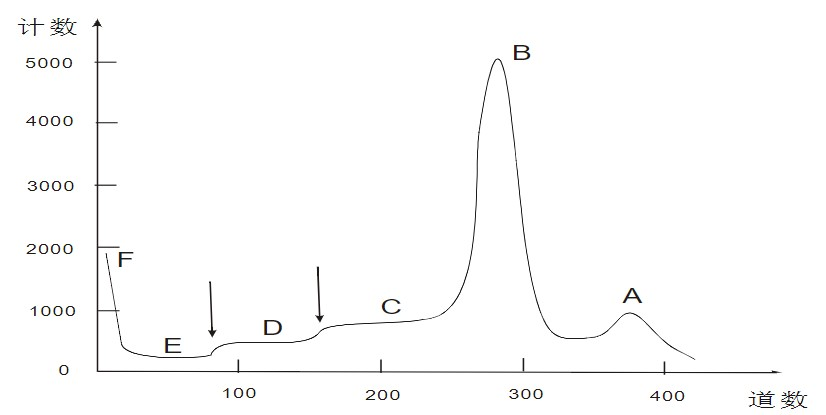
\includegraphics[width=0.9\textwidth]{./fig1.jpg}
        \caption{$BF_3$正比计数管的脉冲幅度谱}
    \end{minipage}
\end{figure}

图中有几个典型的以下区域:

\begin{itemize}
    \item 峰A:对应$6\%$分支,$^{10}B + n \rightarrow ^{7}Li + \alpha + 2.79MeV $
    \item 峰B:对应$94\%$分支,$^{10}B + n \rightarrow ^{7}Li^{\star} + \alpha + 2.31MeV $,$^{7}Li^{\star} \rightarrow ^{7}Li + \gamma(0.48MeV)$
    \item 平台区C,由于核反应发生在计数管近壁区的壁效应所致
    \item 平台区D,由于核反应发生在计数管近壁区的壁效应所致
    \item 平坦低谷区E,由于核反应发生在计数管近壁区的壁效应所致
    \item 平坦低谷区F,是由于探测器噪声和射线在管内转换成的电子产生的低幅度事件造成的(对于噪声水平高的前级放大器的探测系统,F区还包含着电子学噪声).
    但$BF_3$正比计数管用简单的幅度甄别方法可以方便地将$\gamma$本底去掉
\end{itemize}

\subsection{$BF_3$正比计数管的高压坪曲线和甄别阈曲线}

高压坪曲线是探测器计数系统的甄别阈固定时,计数率随高压变化的关系曲线。
甄别阈曲线是高压固定时,计数率随甄别阈改变的关系曲线。
探测器的脉冲幅度谱决定了甄别阈曲线及高压坪曲线的形状,如下图所示。

\begin{figure}[H]
    \centering
    \begin{minipage}[b]{1\textwidth}
        \centering
        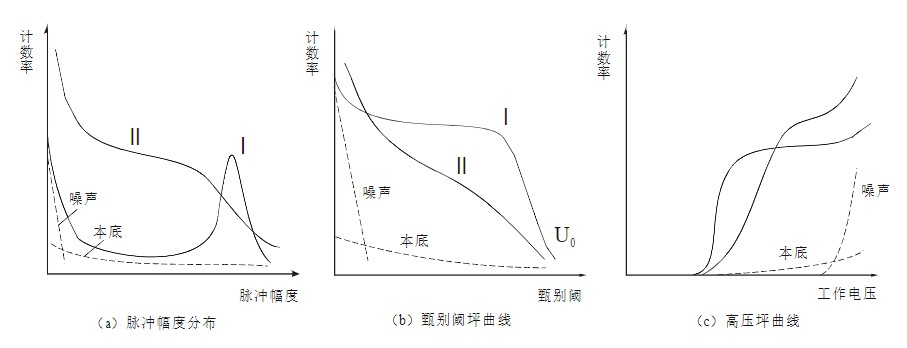
\includegraphics[width=0.9\textwidth]{./fig2.jpg}
        \caption{坪曲线与脉冲幅度谱的关系}
    \end{minipage}
\end{figure}

如果幅度分布谱为曲线I是单峰脉冲分布,相应的甄别阈曲线和高压坪曲线都将有一段坪区:
单峰区和低幅度高计数区之间的低计数区越长,坪越长;此区的计数越少,坪斜越小。

如果幅度分布谱为曲线II是连续脉冲分布,相应的甄别阈曲线和高压坪曲线都没有坪区。
$BF_3$正比计数管的脉冲分布谱决定了它的高压坪曲线和甄别阈曲线的形状。

\section{实验内容}

\begin{figure}[H]
    \centering
    \begin{minipage}[b]{0.9\textwidth}
        \centering
        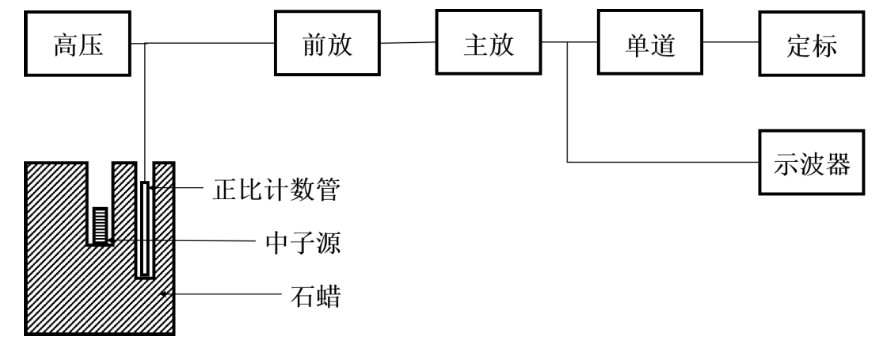
\includegraphics[width=0.9\textwidth]{./fig3.jpg}
        \caption{实验装置示意图}
    \end{minipage}
\end{figure}

用此套装置测量两条甄别阈—计数率曲线以及正比计数管的高压—计数率曲线。

大致实验流程:

\begin{enumerate}
    \item 先选择一个合适的甄别阈电压$1V$,然后调节工作电压,测量计数率。
    \item 再选择一个合适的工作电压,然后调节甄别阈电压,测量计数率。
    \item 最后再选择一个合适的甄别阈电压,然后调节工作电压,测量计数率。
\end{enumerate}

\section{原始数据}

\begin{table}[H]
    \centering
    \caption{甄别阈电压为$1V$时,工作电压与计数率关系表}
    \begin{tabular}{|c|c|c|c|}
    \hline
        \textbf{工作电压U/V} & \textbf{计数率} & \textbf{工作电压U/V} & \textbf{计数率} \\ \hline
        1110 & 60 & 1440 & 42785 \\ \hline
        1140 & 456 & 1470 & 43763 \\ \hline
        1170 & 1436 & 1500 & 43781 \\ \hline
        1200 & 9364 & 1590 & 43975 \\ \hline
        1230 & 25284 & 1680 & 43874 \\ \hline
        1260 & 31362 & 1770 & 44539 \\ \hline
        1290 & 34801 & 1800 & 44534 \\ \hline
        1320 & 37504 & 1830 & 46244 \\ \hline
        1350 & 39588 & 1860 & 59617 \\ \hline
        1380 & 40480 & 1890 & 71035 \\ \hline
        1410 & 42091 & 1920 & 75809 \\ \hline
    \end{tabular}
\end{table}

\begin{table}[H]
    \centering
    \caption{工作电压为$1590V$时,甄别阈电压与计数率关系表}
    \begin{tabular}{|c|c|c|c|}
    \hline
        \textbf{甄别阈电压U/V} & \textbf{计数率} & \textbf{甄别阈电压U/V} & \textbf{计数率} \\ \hline
        0.2 & 107276 & 2.0 & 42325 \\ \hline
        0.25 & 92720 & 2.1 & 42438 \\ \hline
        0.3 & 57416 & 2.2 & 41844 \\ \hline
        0.35 & 45348 & 2.3 & 41500 \\ \hline
        0.4 & 44630 & 2.4 & 41044 \\ \hline
        0.5 & 43917 & 2.5 & 40858 \\ \hline
        0.6 & 43827 & 2.7 & 39828 \\ \hline
        0.7 & 44198 & 2.9 & 39110 \\ \hline
        0.8 & 43813 & 3.1 & 37817 \\ \hline
        0.9 & 44131 & 3.2 & 37619 \\ \hline
        1.0 & 43951 & 3.4 & 36247 \\ \hline
        1.1 & 43920 & 3.6 & 34490 \\ \hline
        1.2 & 44035 & 3.8 & 33161 \\ \hline
        1.3 & 43714 & 4.0 & 31054 \\ \hline
        1.4 & 43803 & 4.2 & 28859 \\ \hline
        1.5 & 43644 & 4.4 & 26234 \\ \hline
        1.6 & 43395 & 4.6 & 21892 \\ \hline
        1.7 & 43237 & 4.8 & 13714 \\ \hline
        1.8 & 43118 & 5.0 & 4529 \\ \hline
        1.9 & 42658 & ~ & ~ \\ \hline
    \end{tabular}
\end{table}

\begin{table}[!ht]
    \centering
    \caption{甄别阈电压为$0.8V$时,工作电压与计数率关系表}
    \begin{tabular}{|c|c|c|c|}
    \hline
        \textbf{工作电压U/V} & \textbf{计数率} & \textbf{工作电压U/V} & \textbf{计数率} \\ \hline
        1110 & 1660 & 1440 & 43887 \\ \hline
        1140 & 8515 & 1470 & 43466 \\ \hline
        1170 & 22799 & 1560 & 43720 \\ \hline
        1200 & 30314 & 1650 & 43738 \\ \hline
        1230 & 34289 & 1680 & 44346 \\ \hline
        1260 & 36961 & 1710 & 43715 \\ \hline
        1290 & 38956 & 1740 & 44137 \\ \hline
        1320 & 40394 & 1770 & 44474 \\ \hline
        1350 & 41383 & 1800 & 46501 \\ \hline
        1380 & 42340 & 1830 & 65039 \\ \hline
        1410 & 43227 & 1860 & 73170 \\ \hline
    \end{tabular}
\end{table}

\section{数据分析}

\begin{figure}[H]
    \centering
    \begin{minipage}[b]{0.9\textwidth}
        \centering
        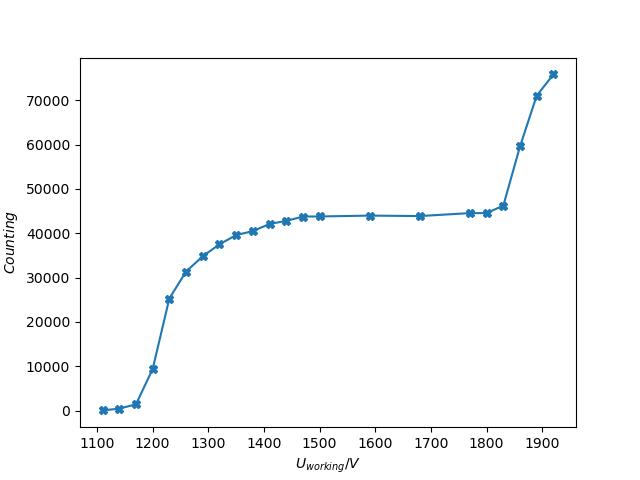
\includegraphics[width=0.9\textwidth]{./ffig1.png}
        \caption{甄别阈电压为$1V$时,工作电压-计数率图}
    \end{minipage}
\end{figure}

可以得到:此时坪长为330V,坪斜为$5.8(\%/100V)$。
此时选择高压坪电压的中值电压$1590V$,作为下一个实验的工作电压。

\begin{figure}[H]
    \centering
    \begin{minipage}[b]{0.9\textwidth}
        \centering
        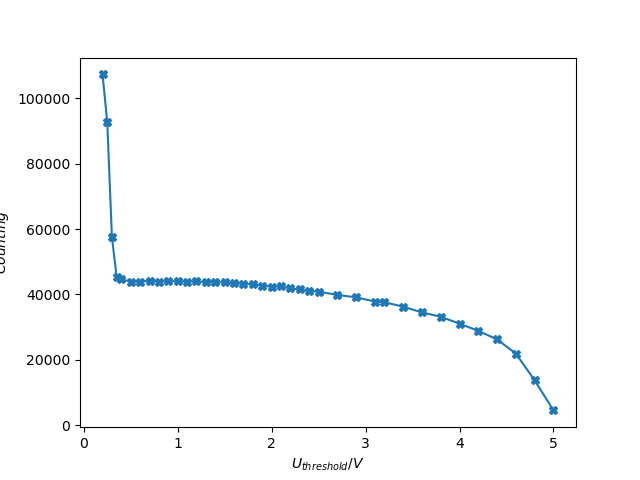
\includegraphics[width=0.9\textwidth]{./ffig2.png}
        \caption{工作电压为$1590V$时,甄别阈电压-计数率图}
    \end{minipage}
\end{figure}

此时选择甄别阈电压较平缓一段的中值电压$0.8V$,作为下一个实验的甄别阈电压。

\begin{figure}[H]
    \centering
    \begin{minipage}[b]{0.9\textwidth}
        \centering
        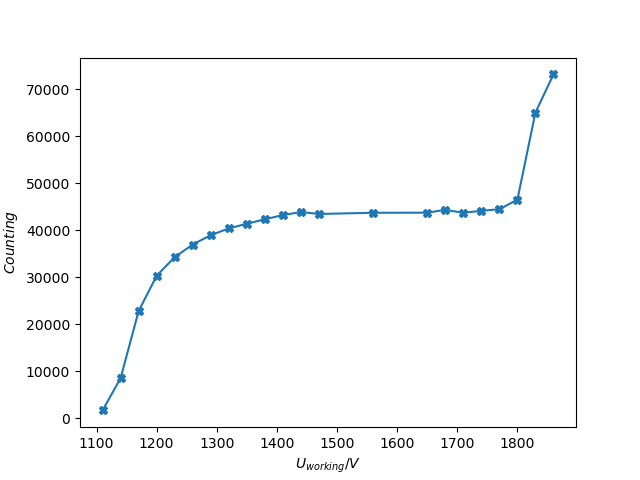
\includegraphics[width=0.9\textwidth]{./ffig3.png}
        \caption{甄别阈电压为$0.8V$时,工作电压-计数率图}
    \end{minipage}
\end{figure}


可以得到:此时坪长为330V,坪斜为$0.4(\%/100V)$。

\section{实验总结}

通过先选择一个合适的甄别阈电压,测量工作电压与计数率的关系,再选择一个合适的工作电压,测量甄别阈电压与计数率的关系,最后再选择一个合适的甄别阈电压,
我们就得到了$BF_3$正比计数管的一对比较合适的甄别阈电压和高压的工作条件。

\section{思考题}

\subsection{什么因素使$BF_3$正比管有这么好的坪长和坪斜?哪些因素影响$2.31MeV$峰的分辨率?}

$BF_3$正比计数管具有良好的坪长和坪斜的原因有几个因素:
\begin{enumerate}
    \item 选择的工作电压:通过适当选择正比计数管的工作电压,可以实现较长的坪长和坪斜。在实验中,通过调节高压以获得合适的工作电压,使得甄别阈曲线和高压坪曲线的坪区达到理想状态。
    \item 甄别阈设置:正确选择甄别阈值可以影响坪长和坪斜的表现。通过实验中选取合适的甄别阈值,可以使得计数率在坪区内保持稳定。
    \item 设备设计和制造:BF3正比计数管的设计和制造过程中考虑了坪长和坪斜的要求。优化的结构和材料选择可提供更好的性能。
\end{enumerate}
影响2.31MeV峰的分辨率的因素有:
\begin{enumerate}
    \item 能量刻度:准确的能量刻度对于峰的位置和分辨率至关重要。能量刻度是通过使用已知能量的标准样品进行校准来实现的。如果能量刻度不准确,峰的位置和宽度可能会受到影响。
    \item 计数统计:峰的分辨率与统计误差有关。更多的计数意味着更好的统计精度,从而提高了分辨率。因此,为了获得更好的2.31MeV峰的分辨率,需要收集足够数量的事件。
    \item 探测器性能:探测器的能量分辨能力也会对峰的分辨率产生影响。性能更好的探测器通常具有更好的能量分辨能力,可以更好地区分不同能量的粒子。探测器性能:探测器的能量分辨能力也会对峰的分辨率产生影响。性能更好的探测器通常具有更好的能量分辨能力,可以更好地区分不同能量的粒子。
    \item 背景噪声:背景噪声的存在可能会降低峰的分辨率。减小背景噪声的方法包括提高探测器的抗干扰能力,优化实验环境等。
\end{enumerate}

\subsection{脉冲幅度谱的能量分辨率和计数系统的甄别阈以及高压坪曲线的坪长有什么内在联系?}

这些参数之间的关系是:较好的能量分辨率通常需要较低的甄别阈和较长的高压坪曲线的坪长。较低的甄别阈使得探测器对较低能量的信号更敏感,可以提高能量分辨率。而较长的坪区表示在一定能量范围内,探测器的计数率变化较小,有利于提高能量分辨率。

\begin{enumerate}
    \item 能量分辨率:脉冲幅度谱的能量分辨率是指探测器对不同能量的粒子或辐射的分辨能力。它反映了探测器能够将不同能量的输入信号区分开的程度。能量分辨率越高,探测器能够更准确地确定入射粒子或辐射的能量。
    \item 甄别阈:甄别阈是指在计数系统中设置的信号幅度阈值,用于区分有效信号和噪声或背景信号。甄别阈的选择可以影响到计数系统的灵敏度和选择性。较低的甄别阈可以提高灵敏度,但也可能导致更多的噪声被识别为有效信号。
    \item 高压坪曲线的坪长:高压坪曲线是指在一定甄别阈下,计数率随高压变化的关系曲线。坪长是指曲线中计数率保持相对稳定的平台区域的长度。坪区的长度取决于探测器的性能和工作状态。较长的坪区表示计数率在一定范围内变化较小,即探测器对入射粒子或辐射的响应相对稳定。
\end{enumerate}

\subsection{计算 30 keV 中子的 $^{10}B (n, \alpha)$ 截面值,并画出你预期的 30 keV 
中子产生的带电粒子脉冲幅度谱,和热中子产生的脉冲幅度谱有多大差别。
从而了解 $BF_3$ 正比管的脉冲谱并不是中子能量谱(注意区别中子能量谱和热中子产生的带电粒子脉冲幅度谱)
。如要探测快中子,$BF_3$ 计数管要加上石蜡外套,即 $BF_3$ 长计数管。}

本实验未涉及这部分内容

\end{document}